\documentclass[t]{beamer}
\usetheme{Copenhagen}
\setbeamertemplate{headline}{} % remove toc from headers
\beamertemplatenavigationsymbolsempty

\usepackage{amsmath, array, tikz, bm, pgfplots, tcolorbox, graphicx,multirow}
\pgfplotsset{compat = 1.16}
\usepgfplotslibrary{statistics}
\usetikzlibrary{trees}

\title{Probability: AND}
\author{}
\date{}

\AtBeginSection[]
{
  \begin{frame}
    \frametitle{Objectives}
    \tableofcontents[currentsection]
  \end{frame}
}

\begin{document}

\begin{frame} 
\maketitle
\end{frame}

\section{Calculate probabilities using the Multiplication Rule}

\begin{frame}{Example 1}
You flip a coin and then roll a single die. What is the probability that you flip heads {\color{blue}\textbf{and}} roll a 5?	\newline\\	
\onslide<2->{
Sample space:	\newline\\
\begin{center}
\begin{tabular}{c|cccccc}
 & \textbf{1} & \textbf{2} & \textbf{3} & \textbf{4} & \textbf{5} & \textbf{6} \\ \hline
\textbf{Heads} & H1 & H2 & H3 & H4 & H5 & H6 \\
\textbf{Tails} & T1 & T2 & T3 & T4 & T5 & T6 
\end{tabular}
\end{center}}
\onslide<3->{\[P(\text{heads and 5}) = \frac{1}{12}\]}
\end{frame}

\begin{frame}{Multiplication Rule}
In the previous example, the probability of flipping heads was $\frac{1}{2}$	\newline\\	\pause
The probability of rolling a 5 was $\frac{1}{6}$	\newline\\	\pause
\begin{tcolorbox}[colframe=green!20!black, colback = green!30!white,title=\textbf{Multiplication Rule}]
If $P(A)$ is the probability of event $A$ occurring, and $P(B)$ is the probability of event $B$ occurring, then
\[P(A\text{ and } B) = P(A) \times P(B)\]
\end{tcolorbox}
\end{frame}

\begin{frame}{Tree Diagram}
\begin{center}
\tikzstyle{level 1} = [level distance = 3cm, sibling distance = 10cm]
\tikzstyle{level 2} = [level distance = 3cm, sibling distance = 1.25cm]
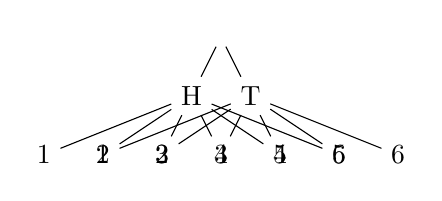
\begin{tikzpicture}[scale=0.5]
\node {}
	child {node {H}
		child {node {1}}
		child {node {2}}
		child {node {3}}
		child {node {4}}
		child {node {5}}
		child {node {6}}}
	child {node {T}{
		child {node {1}}
		child {node {2}}
		child {node {3}}
		child {node {4}}
		child {node {5}}
		child {node {6}} }
		};
\end{tikzpicture}
\end{center}
\end{frame}

\begin{frame}{Venn Diagram -- AND}
\begin{center}
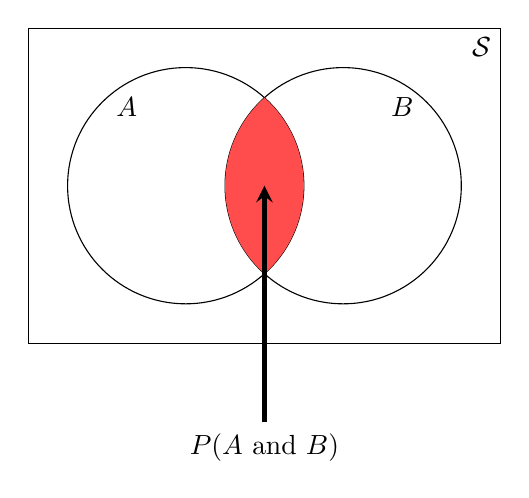
\begin{tikzpicture}
\def\circleA{(2,2) circle [radius = 1.5cm]} 
\def\circleB{(4,2) circle [radius = 1.5cm]} 
\draw (0,0) rectangle (6,4) node [below left] {$\mathcal{S}$};
\draw \circleA;
\node at (1.25,3) {$A$};
\draw \circleB;
\node at (4.75,3) {$B$};
\begin{scope}
\clip \circleA;
\fill[red!70] \circleB;
\end{scope}
\draw [<-, >=stealth, ultra thick] (3,2) -- (3,-1) node [below] {$P(A\text{ and } B)$};
\end{tikzpicture}
\end{center}
\end{frame}

\begin{frame}{Venn Diagram -- AND}
\begin{center}
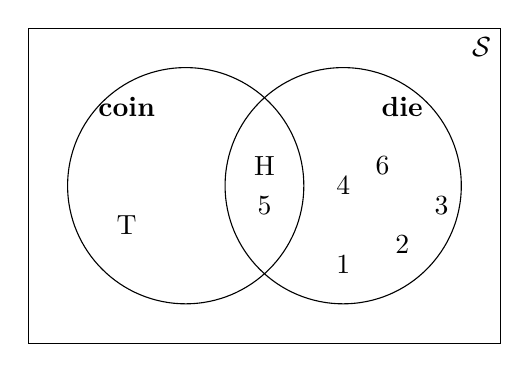
\begin{tikzpicture}
\def\circleA{(2,2) circle [radius = 1.5cm]} 
\def\circleB{(4,2) circle [radius = 1.5cm]} 
\draw (0,0) rectangle (6,4) node [below left] {$\mathcal{S}$};
\draw \circleA;
\node at (1.25,3) {\textbf{coin}};
\draw \circleB;
\node at (4.75,3) {\textbf{die}};
\node at (1.25,1.5) {T};
\node at (3,2.25) {H};
\node at (3,1.75) {5};
\node at (4,1) {1};
\node at (4.75,1.25) {2};
\node at (5.25,1.75) {3};
\node at (4,2) {4};
\node at (4.5,2.25) {6};
\end{tikzpicture}
\end{center}
\end{frame}


\begin{frame}{Mutually Exclusive Events}
\begin{tcolorbox}[colframe=green!20!black, colback = green!30!white,title=\textbf{Mutually Exclusive Events}]
Two events are \textbf{mutually exclusive} if they can not happen together. In other words,
\[P(A\text{ and } B) = 0\]
\end{tcolorbox}
\end{frame}


\section{Find probabilities of independent events}


\begin{frame}{Independent Events}
\begin{tcolorbox}[colframe=green!20!black, colback = green!30!white,title=\textbf{Independent Events}]
Two events are \textbf{independent} if the outcome of the second is not affected by the first happening.
\end{tcolorbox}
\vspace{8pt} 

\onslide<2->{\[P(A \text{ and } B) = P(A) \times P(B)\]}

\onslide<3->{When selecting items from a collection, independent events often contain selections made \alert{\underline{with replacement}}.}
\end{frame}

\begin{frame}{Example 2}
A jar contains 10 blue, 12 black, and 15 red marbles.	\newline\\
(a)	\quad What is the probability of selecting a black marble, putting it back, and then selecting a blue marble?
\begin{align*}
	\onslide<2->{P(\text{black and blue}) &= \frac{12}{37} \times \frac{10}{37}} \\[8pt]
	\onslide<3->{&= \frac{120}{1,369}}
\end{align*}
\end{frame}

\begin{frame}{Example 2}

A jar contains 10 blue, 12 black, and 15 red marbles.	\newline\\
(b)	\quad What is the probability of selecting a red marble, putting it back, and then selecting another red marble?
\begin{align*}
	\onslide<2->{P(\text{red and red}) &= \frac{15}{37} \times \frac{15}{37}} \\[8pt]
	\onslide<3->{&= \frac{225}{1,369}}
\end{align*}
\end{frame}

\section{Find conditional probabilities}

\begin{frame}{Conditional Probability}
\begin{tcolorbox}[colframe=green!20!black, colback = green!30!white,title=\textbf{Conditional Probability}]
\textbf{Conditional probability} is found by determining a probability \emph{based on a previous event happening}.
\end{tcolorbox}
\vspace{8pt} 

\onslide<2->{The notation for the probability that event $B$ occurs given that event $A$ has occurred is
\[ P(B \mid A)\]}
\onslide<3->{With conditional probability, the denominator will often by the total of something that follows the words ``if", ``suppose that", or ``given that".}
\end{frame}

\begin{frame}{Example 3}
The table below lists the types and numbers of cars sold at Lemon Autos along with their ages. Find each probability.	\newline\\
\begin{center}
\begin{tabular}{c|ccccc}
					&	\textbf{0--2} & \textbf{3--5} & \textbf{6--10} & \textbf{Over 10} & \textbf{Total} \\ \hline
\textbf{Foreign} 	& 37 & 21 & 12 & 30 & 100 \\
\textbf{Domestic} 	& 35 & 23 & 11 & 31 & 100 \\ \hline
\textbf{Total}   	& 72 & 44 & 23 & 61 & 200
\end{tabular}
\end{center}
(a) If a domestic car is randomly selected, what is the probability that it is 6--10 years old?	
\begin{align*}
\onslide<2->{P(\text{6--10 years old given that it is a domestic car}) &= \frac{12}{100}}	\\[8pt]
\onslide<3->{&= \frac{3}{25}}
\end{align*}
\end{frame}

\begin{frame}{Example 3}
\begin{center}
\begin{tabular}{c|ccccc}
					&	\textbf{0--2} & \textbf{3--5} & \textbf{6--10} & \textbf{Over 10} & \textbf{Total} \\ \hline
\textbf{Foreign} 	& 37 & 21 & 12 & 30 & 100 \\
\textbf{Domestic} 	& 35 & 23 & 11 & 31 & 100 \\ \hline
\textbf{Total}   	& 72 & 44 & 23 & 61 & 200
\end{tabular}
\end{center}
(b) What is the probability of selecting a domestic car given that the car is 6--10 years old?	
\begin{align*}
\onslide<2->{P(\text{domestic car given that it is 6--10 years old}) &= \frac{11}{23}}
\end{align*}
\end{frame}

\begin{frame}{Example 3}
\begin{center}
\begin{tabular}{c|ccccc}
					&	\textbf{0--2} & \textbf{3--5} & \textbf{6--10} & \textbf{Over 10} & \textbf{Total} \\ \hline
\textbf{Foreign} 	& 37 & 21 & 12 & 30 & 100 \\
\textbf{Domestic} 	& 35 & 23 & 11 & 31 & 100 \\ \hline
\textbf{Total}   	& 72 & 44 & 23 & 61 & 200
\end{tabular}
\end{center}
(c) Suppose that a new car is selected, what is the probability that it is a foreign car?	
\begin{align*}
\onslide<2->{P(\text{foreign car given that it is 0--2 years old}) &= \frac{37}{72}}
\end{align*}
\end{frame}

\section{Find probabilities of dependent events}

\begin{frame}{Dependent Events}
\begin{tcolorbox}[colframe=green!20!black, colback = green!30!white,title=\textbf{Dependent Events}]
Two events are \textbf{dependent} if the outcome of the second is affected by the first happening.
\end{tcolorbox}
\vspace{8pt}	\pause

When selecting items from a collection, dependent events often contain selections made \alert{\underline{without replacement}}.
\end{frame}

% Dependent Events

\end{document}
